\documentclass[12pt, a4paper, oneside]{ctexart}
\usepackage{amsmath, amsthm, amssymb, bm, color, graphicx, geometry, mathrsfs,extarrows, braket, booktabs, array, wrapfig, enumitem}
\usepackage[colorlinks,linkcolor=red,anchorcolor=blue,citecolor=blue,urlcolor=blue,menucolor=black]{hyperref}
\setCJKmainfont{方正新书宋_GBK.ttf}[ BoldFont = 方正小标宋_GBK, ItalicFont = 方正楷体_GBK]
\setmainfont{Times New Roman}  % 设置英文字体
\setsansfont{Calibri}
\setmonofont{Consolas}

\linespread{1.4}
%\geometry{left=2.54cm,right=2.54cm,top=3.18cm,bottom=3.18cm}
\geometry{left=1.84cm,right=1.84cm,top=2.18cm,bottom=2.18cm}
\newcounter{problem}  % 问题序号计数器
\newenvironment{problem}[1][]{\stepcounter{problem}\par\noindent\textbf{题目\arabic{problem}. #1}}{\smallskip\par}
\newenvironment{solution}[1][]{\par\noindent\textbf{#1解答. }}{\smallskip\par}  % 可带一个参数表示题号\begin{solution}{题号}
\newenvironment{note}{\par\noindent\textbf{注记. }}{\smallskip\par}

%%%% 图片相对路径 %%%%
\graphicspath{{figure/}} % 当前目录下的figure文件夹, {../figure/}则是父目录的figure文件夹

%%%% 缩小item,enumerate,description两行间间距 %%%%
\setenumerate[1]{itemsep=0pt,partopsep=0pt,parsep=\parskip,topsep=5pt}
\setitemize[1]{itemsep=0pt,partopsep=0pt,parsep=\parskip,topsep=5pt}
\setdescription{itemsep=0pt,partopsep=0pt,parsep=\parskip,topsep=5pt}

\everymath{\displaystyle} % 默认全部行间公式
\DeclareMathOperator*\uplim{\overline{lim}} % 定义上极限 \uplim_{}
\DeclareMathOperator*\lowlim{\underline{lim}} % 定义下极限 \lowlim_{}
\let\leq=\leqslant % 将全部leq变为leqslant
\let\geq=\geqslant % geq同理

%%%% 一些宏定义 %%%%
\def\bd{\boldsymbol}        % 加粗(向量) boldsymbol
\def\disp{\displaystyle}    % 使用行间公式 displaystyle(默认)
\def\tsty{\textstyle}       % 使用行内公式 textstyle
\def\sign{\text{sign}}      % sign function
\def\wtd{\widetilde}        % 宽波浪线 widetilde
\def\R{\mathbb{R}}          % Real number
\def\N{\mathbb{N}}          % Natural number
\def\Z{\mathbb{Z}}          % Integer number
\def\Q{\mathbb{Q}}          % Rational number
\def\C{\mathbb{C}}          % Complex number
\def\K{\mathbb{K}}          % Number Field
\def\P{\mathbb{P}}          % Polynomial
\def\d{\mathrm{d}}          % differential operator
\def\e{\mathrm{e}}          % Euler's number
\def\i{\mathrm{i}}          % imaginary number
\def\re{\mathrm{Re}}        % Real part
\def\im{\mathrm{Im}}        % Imaginary part
\def\res{\mathrm{Res}}      % Residue
\def\ker{\mathrm{Ker}}      % Kernel
\def\L{\mathcal{L}}         % Loss function
\def\wdh{\widehat}          % 宽帽子 widehat
\def\ol{\overline}          % 上横线 overline
\def\ul{\underline}         % 下横线 underline
\def\add{\vspace{1ex}}      % 增加行间距
\def\del{\vspace{-1.5ex}}   % 减少行间距

%%%% 定理类环境的定义 %%%%
\newtheorem{theorem}{定理}

%%%% 基本信息 %%%%
\newcommand{\RQ}{\today} % 日期
\newcommand{\km}{泛函分析} % 科目
\newcommand{\bj}{强基数学002} % 班级
\newcommand{\xm}{吴天阳} % 姓名
\newcommand{\xh}{2204210460} % 学号

\begin{document}

%\pagestyle{empty}
\pagestyle{plain}
\vspace*{-15ex}
\centerline{\begin{tabular}{*5{c}}
    \parbox[t]{0.25\linewidth}{\begin{center}\textbf{日期}\\ \large \textcolor{blue}{\RQ}\end{center}} 
    & \parbox[t]{0.2\linewidth}{\begin{center}\textbf{科目}\\ \large \textcolor{blue}{\km}\end{center}}
    & \parbox[t]{0.2\linewidth}{\begin{center}\textbf{班级}\\ \large \textcolor{blue}{\bj}\end{center}}
    & \parbox[t]{0.1\linewidth}{\begin{center}\textbf{姓名}\\ \large \textcolor{blue}{\xm}\end{center}}
    & \parbox[t]{0.15\linewidth}{\begin{center}\textbf{学号}\\ \large \textcolor{blue}{\xh}\end{center}} \\ \hline
\end{tabular}}
\begin{center}
    \zihao{-3}\textbf{第八次作业}
\end{center}
\vspace{-0.2cm}
% 正文部分
\begin{problem}[(2.3.1)]
    设$X$为$B$空间,$X_0$是$X$的闭子空间. 映射$\varphi:X\to X/X_0$定义为$\varphi:x\mapsto[x],\ (\forall x\in X)$,其中$[X]$表示$x$的商类. 证明$\varphi$是开映射.
\end{problem}
\begin{proof}
    由开映射定理可知,只需证$X/X_0$是完备的. 令$\{[x_n]\}\subset X/X_0$是Cauchy列,则存在子列$\{[x_{n_k}]\}$使得$||[x_{n_{k+1}}]-[x_{n_k}]|| = ||[x_{n_{k+1}}-x_{n_k}]||\leq 1/2^k$,由商空间范数定义可知,$\forall \varepsilon > 0$,$\exists y_k\in X_0$使得$||x_{n_{k+1}}-x_{n_{k}}+y_k|| < ||[x_{n_{k+1}}-x_{n_{k}}]||+\varepsilon\leq 1/2^k+\varepsilon$,则$||x_{n_{k+1}}-x_{n_{k}}+y_k|| < 1/2^k$,于是$\sum_{k=1}^\infty ||x_{n_{k+1}}-x_{n_{k}}+y_k|| < \sum_{k=1}^\infty\frac{1}{2^k}=1$绝对收敛,由于$X$是完备的,则$\sum_{k=1}^\infty x_{n_{k+1}}-x_{n_{k}}+y_k$收敛,令部分和$\{x_{n_{k+1}}+\sum_{i=1}^ky_i\}$收敛到$x+y,\ x\in X, y\in X_0$,由$\varphi$的连续性可得$\lim_{n\to\infty}[x_n] = \lim_{n\to\infty}\left[x_{n_k}+\sum_{i=1}^{k-1}y_i\right] = [x+y] = [x]\in X/X_0$,所以$X/X_0$是商空间.
\end{proof}
\begin{problem}[(2.3.2)]
    设$X,Y$是$B$空间,又设方程$Ux=y$对$\forall y\in Y$有解$x\in X$,其中$U\in L(X,Y)$,并且$\exists m  > 0$,使得$||Ux|| \geq m||x||,\ (\forall x\in X)$,求证:$U$有连续逆$U^{-1}$,并且$||U^{-1}||\leq 1/m$.
\end{problem}
\begin{proof}
    由条件可知$U$是满射,假设$\exists x_1,x_2\in X$使得$Ux_1=Ux_2$,则$U(x_1-x_2) = \theta\Rightarrow x_1=x_2$,于是$U$是单射,故$U$是双射.

    由逆算子定理可知$U^{-1}\in L(Y,X)$,由于$||Ux||\geq m||x||$,令$x = U^{-1}y$得$||y||\geq m||U^{-1}y||$,则$||U^{-1}y||\leq ||y||/m,\ (\forall y\in Y)$,则$||U^{-1}||\leq 1/m$.
\end{proof}
\begin{problem}[(2.3.3)]
    设$H$为Hilbert空间,$A\in L(H)$,且$\exists m > 0$,使得$|(Ax,x)|\geq m||x||^2,\ (\forall x\in H)$. 求证:$\exists A^{-1}\in L(H)$.
\end{problem}
\begin{proof}
    由逆算子定理知,只需证$A$为双射. 假设$\exists y_1,y_2\in X$使得$Ay_1=Ay_2$则
    \begin{equation*}
        m||y_1-y_2||^2\leq |(A(y_1-y_2),y_1-y_2)| = |(\theta,(y_1-y_2))| = 0\Rightarrow y_1=y_2
    \end{equation*}
    故$A$是单射. 
    
    下证$R(A)=Y$,只需证$R(A)$是闭的且$R(A)^\perp = \{\theta\}$. 设$\{Ax_n\}\subset H$收敛于$y\in H$,由于
    \begin{equation*}
        m||x||^2\leq |(Ax,x)|\leq ||Ax||\cdot||x||\Rightarrow m||x||\leq ||Ax||
    \end{equation*}
    于是$||x_{n+p}-x_n||\leq ||Ax_{n+p}-Ax_n||\to 0,\ (n\to\infty,\forall p>0)$则$\{x_n\}$为Cauchy列,由于$H$完备,令其收敛于$x$,由$A$的连续性可得$Ax=y\in R(A)$,所以$A$是闭的. 令$x_0\in R(A)^\perp$则$||x_0||^2\leq ||(Ax_0,x_0)||/m = 0\Rightarrow x_0 = \theta$则$\R(A)^\perp = \{\theta\}$,于是$\overline{R(A)} = R(A) = Y$. 所以$A$是满射.

    综上,$A$是双射.
\end{proof}
\begin{problem}[(2.3.4)]
    设$X,Y$是$B^*$空间,$D$是$X$的线性子空间,且$A:D\to Y$是线性映射. 求证:
    
    (1). 若$A$连续且$D$是闭的,则$A$是闭算子.

    (2). 若$A$连续且是闭算子,则$Y$完备蕴含$D$是闭的.

    (3). 若$A$是单射的闭算子,则$A^{-1}$也是闭算子.

    (4). 若$X$完备,$A$是单射的闭算子,$R(A)$在$Y$中稠密,且$A^{-1}$连续,那么$R(A) = Y$.
\end{problem}
\begin{proof}
    (1). $\forall \{x_n\}\subset D$满足$x_n\to x,\ Ax_n\to y$,由于$D$是闭的可得$x\in D$,由$A$连续性可得$Ax_n\to Ax = y$,所以$A$是闭算子.

    (2). 反设$D$是开的,则$\exists x_0\in X\setminus D,\ \{x_n\}\subset D$使得$x_n\to x_0$,由于
    \begin{equation*}
        ||Ax_{n+p}-Ax_n||\leq ||A||\cdot ||x_{n+p}-x_n||\to 0,\ (n\to\infty,\ \forall p > 0)
    \end{equation*}
    则$\{Ax_n\}$是$Y$中的Cauchy列,令$\lim_{n\to\infty}Ax_n = y$,由于$A$为闭算子,则$x\in D$,这与$x\in X\setminus D$矛盾. 故$D$是闭的.

    (3). 由于$A$是单射,则$A^{-1}$有意义,$\forall \{y_n\}\subset R(A)$满足$y_n\to y,\ A^{-1}y_n\to x$,由$A$是闭算子,则$A^{-1}y_n\to A^{-1}y,\ y_n\to Ax$可得到$A^{-1}y\in D$且$A(A^{-1}y)=y=Ax$,于是$y\in R(A)$且$A^{-1}y\in X$.

    (4). 由(3)可知,$A^{-1}$是闭算子,由(2)可知$X$完备且$A^{-1}$连续,则$R(A)$是闭的,又由于$R(A)$在$Y$中稠密,则$R(A) = \ol{R(A)} = Y$.
\end{proof}
\begin{problem}[(2.3.5)]
    用等价范数定理证明:$(C[0,1],||\cdot||_1)$不是$B$空间.
\end{problem}
\begin{proof}
    若$(C[0,1],||\cdot||_1)$是$B$空间,由等价模定理可知$||\cdot||_1$与$||\cdot ||_{\infty}$等价. 令$x_n = t^{1/n},\ x = 1$于是
    \begin{align*}
        ||x_n-x||_1 =&\ \int_0^1|x^{1/n}-1|\,\d x = \frac{1}{n+1}\to 0,\ (n\to\infty)\\
        ||x_n-x||_\infty =&\ \max_{0\leq t\leq 1} 1 - t^{1/n} \geq 1-\left(\frac{1}{n^n}\right)^{1/n} = \frac{n-1}{n}\to 1,\ (n\to\infty)
    \end{align*}
    于是$\{x_n\}$在$||\cdot||_1$范数下收敛,但在$||\cdot||_\infty$范数下不收敛,则它们不等价,矛盾. 故$(C[0,1], ||\cdot||_1)$不是$B$空间.
\end{proof}
\begin{problem}[(2.3.6)]
    (Gelfand引理)设$X$为$B$空间,$p:X\to \R$满足
    \begin{enumerate}[label=(\arabic*)]
        \item $p(x)\geq 0,\ (\forall x\in X)$;
        \item $p(\lambda x) = \lambda p(x),\ (\forall \lambda >0, \forall x\in X)$;
        \item $p(x_1+x_2)\leq p(x_1)+p(x_2),\ (\forall x_1,x_2\in X)$;
        \item 当$x_n\to x$时,$\lowlim_{n\to\infty}p(x_n)\geq p(x)$.
    \end{enumerate}
    求证:$\exists M > 0$,使得$p(x)\leq M||x||,\ \forall x\in X$.
\end{problem}
\begin{proof}
    定义$X$上的范数$||x||_G = ||x||+\sup_{|\alpha| = 1}p(\alpha x)$,下面证明$||\cdot ||$是$X$上的范数:
    
    \noindent 正定性:任取$x_0\in X$,则$\frac{x_0}{n}\to \theta$,由假设知$0\leq p(\theta)\leq \lowlim_{n\to\infty}\frac{p(x_0)}{n} = 0$,于是$p(\theta) = 0$. 故$||x||_G = 0\iff x = \theta,\ ||x||_G\geq 0$.

    \noindent 齐次性:不妨令$\K = \C$,$\forall \beta \in \K$,令$\beta = |\beta|\e^{\i \theta}$,由于
    \begin{equation*}
        \sup_{|\alpha| = 1}p(\alpha\beta x) = |\beta|\sup_{|\alpha|=1}p(\alpha\e^{\i\theta}x) = |\beta|\sup_{|\alpha|=1}p(\alpha x)
    \end{equation*}
    则$||\beta x||_G = |\beta|\cdot ||x|| + \sup_{|\alpha|=1}p(\alpha\beta x) = |\beta|\cdot (||x||+\sup_{|\alpha|=1}p(\alpha x)) = |\beta|\cdot ||x||_G$.

    \noindent 三角不等式:由于$||\cdot ||$与$p(x)$分别都满足三角不等式,结合线性性知$||\cdot||_G$满足三角不等式.

    下证$(X,||\cdot||_G)$是$B$空间. 令$\{x_n\}$是$X$中的Cauchy列,则
    \begin{equation*}
        ||x_n-x_m||_G = ||x_n-x_m||+\sup_{|\alpha|=1}p(\alpha(x_n-x_m))\to 0,\ (n,m\to\infty)
    \end{equation*}
    则$x_n-x_m\to 0,\ (n,m\to\infty)$,由于$X$是完备的,则$x_n\to x\in X$,又由于$p(x)\geq 0$,则$\sup_{|\alpha|=1}p(\alpha(x_n-x_m))\to 0,\ (n,m\to\infty)$于是$\forall |\alpha| = 1$有$p(\alpha(x_n-x_m))\to 0$,由于$x_m\to x$,则由假设条件(4)可知
    \begin{equation*}
        p(\alpha(x_n-x))\leq \lowlim_{m\to\infty}p(\alpha(x_n-x_m))\to 0,\ (n\to\infty,\forall |\alpha|=1)
    \end{equation*}
    于是$\sup_{|\alpha|=1}p(\alpha(x_n-x))\to 0,\ (n\to\infty)$.

    综上,$||x_n-x||_G\to 0$,则$(X,||\cdot||_G)$是$B$空间.

    由于$||\cdot||_G\geq ||\cdot||$,由等价模定理可知,$||\cdot||_G\leq ||\cdot||$,于是$\exists M > 0$使得
    \begin{equation*}
        p(x)\leq \sup_{|\alpha|=1}p(\alpha x)\leq ||x||_G\leq M\cdot ||x||
    \end{equation*}
\end{proof}
\begin{problem}[(2.3.7)]
    设$X$和$Y$是$B$空间,$A_n\in L(X,Y),\ (n=1,2,\cdots)$,且$\forall x\in X$,$\{A_nx\}$在$Y$中收敛. 求证:$\exists A\in L(X,Y)$使得
    \begin{equation*}
        A_nx\to Ax,\ (\forall x\in X),\quad \text{且}\quad ||A||\leq \lowlim_{n\to\infty}||A_n||.
    \end{equation*}
\end{problem}
\vspace*{-1cm}
\begin{proof}
    $\forall x \in X$,令$Ax = \lim_{n\to\infty}A_nx$,由于$A_n$为线性泛函,则$A$也具有线性性,由于$\forall x\in X$有$A_nx$收敛,$\sup_{n\geq 1}||A_nx|| < \infty$,由共鸣定理知,$\exists M>0$使得$||A_n||\leq M$. 于是
    \begin{equation*}
        ||Ax|| = \lim_{n\to\infty}||A_nx|| = \lowlim_{n\to\infty}||A_nx||\leq \lowlim_{n\to\infty}||A_n||\cdot ||x||\leq M||x||
    \end{equation*}
\end{proof}
\begin{problem}[(2.3.8)]
    设$1 < p<\infty$,并且$1/p+1/q=1$,若序列$\{\alpha_k\}$使得对$\forall x\in \{\xi_k\} \in l^p$保证$\sum_{k=1}^\infty \alpha_k\xi_k$收敛,求证:$\{\alpha_k\}\in l^q$. 又若$f:x\mapsto \sum_{k=1}^\infty \alpha_k\xi_k$,求证:$f$作为$l^p$上的线性泛函,有$||f|| = ||\alpha||_q$.
\end{problem}
\clearpage
\begin{proof}
    令$f_n(x) = \sum_{1\leq k\leq n}\alpha_k\xi_k,\ (\forall x=\{\xi_k\}\in l^p)$,则$f_n(x)$连续,$f_n\in (l^p)^*$,由于$\{f_nx\}$收敛到$\sum_{k\geq 1}\alpha_k\xi_k =: fx$,由题目2.3.7可知,$f\in(l^p)^*$,令
    \begin{equation*}
        x_0^n = \{\xi_k^n\},\quad \xi_k^n=\begin{cases}
            |\alpha_k|\e^{-\i\theta_k},&\quad k\leq n,\ (\theta_k = \text{arg }\alpha_k)\\
            0,&\quad k > n.
        \end{cases}
    \end{equation*}
    由于$x_0^n$只有有限项不为$0$,则$x_0^n\in l^p$,并且$1/p+1/q=1\Rightarrow (q-1)p = q$,可得
    \begin{align*}
        f(x_0^n) =&\ \sum_{1\leq k\leq n}|\alpha_k|^{q-1}\e^{-\i\theta_k}|\alpha_k|\e^{\i\theta_k} = \sum_{1\leq k\leq n}|\alpha_k|^q\\
        \leq&\ |f(x_0^n)|\leq ||f||\cdot ||x_0^n||_p = ||f||\left(\sum_{1\leq k\leq n}|\alpha_k|^{(q-1)p}\right)^{\frac{1}{p}} = ||f||\left(\sum_{1\leq k\leq n}|\alpha_k|^{q}\right)^{\frac{1}{p}}
    \end{align*}
    则$\left(\sum_{1\leq k\leq n}|\alpha_k|^q\right)^{1-\frac{1}{p}} = \left(\sum_{1\leq k\leq n}|\alpha_k|^q\right)^{\frac{1}{q}}\leq ||f||$. 令$n\to\infty$,可得$\alpha\in l^q$且$||\alpha||_q\leq ||f||$.

    由Holder不等式可得$|f(x)| = |(\alpha, x)| \leq ||\alpha||_{q}||x||_p$,于是$||f||\leq ||\alpha||_q$.

    综上,$||f|| = ||\alpha||_q$.
\end{proof}
\begin{problem}[(2.3.9)]
    若序列$\{\alpha_k\}$使得$\forall x=\{\xi_k\}\in l^1$,保证$\sum_{k\geq 1} \alpha_k\xi_k$收敛,求证:$\{\alpha_k\}\in l^\infty$. 若$f:x\mapsto\sum_{k\geq 1}\alpha_k\xi_k$作为$l^1$上的线性泛函,求证:$||f||=||\alpha||_\infty$.
\end{problem}
\begin{proof}
    令$f_n = \sum_{1\leq k\leq n}\alpha_k\xi_k,\ (\forall x\in\{\xi_k\}\in l^1)$则$f_n\in (l^1)^*$,由题目2.3.7可知,$f_n\to f = \sum_{k\geq 1}\alpha_k\xi_k$且$f\in(l^1)^*$,令$e_k = \{\underbrace{0,0,\cdots,0,1}_{k\text{个}},0,\cdots\}$,则$|\alpha_k| = |f(e_k)| \leq ||f||\cdot ||e_k||_1 = ||f||$,则$|\alpha_k|$有界,故$\alpha\in l^\infty$且$||\alpha||_\infty\leq ||f||$.

    又由于$\forall n\geq 1$,$||f_n(x)||\leq\sum_{1\leq k\leq n}|\alpha_k\cdot |x_k|\leq \sup_{k\geq 1}|\alpha_k|\sum_{1\leq k\leq n}|x_k|\leq ||\alpha||_{\infty}||x||_1$,则$|f(x)| = \lim_{n\to\infty}|f_n(x)|\leq ||\alpha||_{\infty}||x||_1$,于是$||f||\leq ||\alpha||_{\infty}$.

    综上,$||f|| = ||\alpha||_{\infty}$.
\end{proof}
\begin{problem}[(2.3.10)]
    用Gelfand引理(习题2.3.6)证明共鸣定理.
\end{problem}
\begin{proof}
    令$p(x) = \sup_{A\in W}||Ax||$,则$p(x)\geq 0$,$\forall \lambda > 0$,有$p(\lambda x) = \sup_{A\in W}||A\lambda x|| = \lambda\sup_{A\in W}||Ax|| = \lambda p(x)$.
    \begin{equation*}
        p(x_1+x_2) = \sup_{A\in W}||A(x_1+x_2)|| = \sup_{A\in W}||Ax_1+Ax_2||\leq \sup_{A\in W}||Ax_1||+||Ax_2|| = p(x_1)+p(x_2)
    \end{equation*}
    当$x_n\to x$时,由于$\sup_{A\in W}||Ax_n||\geq ||Ax_n||$,则$\lowlim_{n\to\infty}\sup_{A\in W}||Ax_n||\geq \lowlim_{n\to\infty}||Ax_n||,\ (\forall A\in W)$,于是
    \begin{equation*}
        \lowlim_{n\to\infty}p(x) = \lowlim_{n\to\infty}\sup_{A\in W}||Ax_n||\geq \sup_{A\in W}\lowlim_{n\to\infty}||Ax_n|| = \sup_{A\in W}||Ax|| = p(x)
    \end{equation*}

    综上$p(x)$满足Gelfand引理四个条件,于是$\exists M > 0$,使得$||Ax||\leq p(x)\leq M||x||,\ \forall x\in X$,于是$||A||\leq M,\ (\forall A\in W)$.
\end{proof}
\begin{problem}[(2.3.11)]
    设$X,Y$是$B$空间,$A\in L(X,Y)$是满射. 求证:若在$Y$中$y_n\to y_0$,则$\exists C > 0$与$x_n\to x_0$,使得$Ax_n = y_n$,且$||x_n||\leq C||y_n||$.
\end{problem}
\begin{proof}
    \textbf{分析}:由于$A$不一定为单射,但是商空间$X/N(A)$中等价映射是单射,因为如果$Ax=Ay$,则有$x,y\in [x]$,因此商空间的等价算子是双射. 从而得到$||x||$大小可被$||Ax||$控制. 再将$y_n$做平移为$y_n-y_0$收敛到$\theta$,利用开映射定理得到$||x_n||$可被$||y_n||,||y_0||$控制,由于$y_n\to y_0$所以$||y_0||$大小可被$||y_n||$控制,于是$||x_n||$可被$||y_n||$控制.
    
    下面进行证明:令$N(A) = \{x\in X:A(x) = \theta\}$,由于$A$有界,则$N(A)$是$X$的闭子空间,于是商空间$X/N(A)$关于范数$||[x]|| = \inf_{y\in[x]}||y||$构成$B$空间. 令$T:X/N(A)\to Y$为$T[x] = Ax$,由于$\forall x,y\in [x]$有$x-y \in N(A)$,于是$A(x-y) = 0\Rightarrow Ax=Ay\Rightarrow T[x] = T[y]$,所以$T$是一个映射. 下面证明$T$是双射:

    \noindent 单射:$\forall [x],[y]\in X/N(A)$且$T[x] = T[y]$,则$Ax=Ay\Rightarrow A(x-y) = \theta\Rightarrow[x-y] = [\theta]\Rightarrow[x]=[y]$.

    \noindent 满射:由于$A$是满射,则$\forall y\in Y$,$\exists x\in X$使得$Ax=y$,则$T[x] = y$.

    综上$T$是双射,且$||T[x]|| = ||Ax||\leq ||A||\cdot||x||$,则$T$有界,由逆算子定理可知$T^{-1}$有界.

    则$\forall y\in Y$,$\exists [x]\in X/N(A)$,使得$T[x] = y\Rightarrow ||[x]|| = ||T^{-1}y||\leq ||T^{-1}||\cdot ||y||$,由于$||[x_n]|| = \inf_{z\in[x]}||z||$,则$\exists x_0\in [x]$使得$||x_0||\leq 2||[x]||\leq 2||T^{-1}||\cdot ||y||$且$Ax_0 = y$.

    若$y_n=\theta$时,取$x_n = \theta$,所以不妨令下述$y_n\neq \theta$

    令$z_n = y_n-y_0$,则$z_n\to \theta$,由开映射定理$\exists c>0$,\add 使得$B_Y(\theta, c)\subset AB_X(\theta, 1)$,则$B_Y(\theta,2||z_n||)\subset AB_X(\theta,\frac{2||z_n||}{c})$,则$\exists x_n'\in X$且$||x_n'|| < \frac{2||z_n||}{c}$使得$z_n=Ax_n'$,取\add $x_0\in X$使得$Ax_0 = y_0$且$||x_0||\leq 2||T^{-1}||\cdot ||y_0||$,令$x_n = x_n'+x_0$,则$Ax_n = Ax_n'+Ax_0 = y_n-y_0+y_0 = y_n$,且
    \begin{equation*}
        ||x_n|| = ||x_n'+x_0|| \leq \frac{2||y_n-y_0||}{c} + 2||T^{-1}||\cdot ||y_0||\leq \frac{2}{c}||y_n||+2(||T^{-1}||+1/c)||y_0||
    \end{equation*}
    由于$y_n\to y_0$,则$\exists N \in \N$使得$\forall n\geq N$有
    \begin{equation*}
        ||y_0||-||y_n||\leq ||y_0-y_n||\leq \frac{1}{2}||y_0||\Rightarrow||y_0||\leq 2||y_n||
    \end{equation*}
    令$M = \max\biggl\{\{||y_0||/||y_n||:1\leq n\leq N\}, 2\biggl\}$,则$||y_0||\leq M||y_n||$,所以
    \begin{equation*}
        ||x_n||\leq \left[\frac{2}{c}+2M(||T^{-1}||+1/c)\right]||y_n||
    \end{equation*}
\end{proof}
\begin{problem}[(2.3.12)]
    设$X,Y$是$B$空间,$T$是闭线性算子,$D(T)\in X$,$R(T)\in Y$,$N(T):=\{x\in X:Tx=\theta\}$.
    \begin{enumerate}[label=(\arabic*)]
        \item 求证:$N(T)$是$X$的闭线性子空间.
        \item 求证:$N(T)=\{\theta\}$,$R(T)$在$Y$中闭的充要条件为$\exists \alpha >0$,使得
        \begin{equation*}
            ||x||\leq ||\alpha||Tx||,\ (\forall x\in D(T)).
        \end{equation*}
        \item 令$d(x,N(T)):=\inf_{z\in N(T)}||z-x||$. 求证:$R(T)$在$Y$中闭的充要条件为$\exists \alpha >0$使得
        \begin{equation*}
            d(x,N(T))\leq \alpha||Tx||,\ (\forall x\in D(T)).
        \end{equation*}
    \end{enumerate}
\end{problem}
\begin{proof}
    (1). $\forall \{x_n\}\subset N(T)$收敛于$x$,则$Tx_n=\theta$,于是$Tx_n\to y = \theta$,由于$T$是闭的,则$x\in D(T)$且$Tx=y=\theta$,则$x\in N(T)$. 故$N(T)$是闭线性子空间.

    (2). 必要性:由于$N(T) = \{\theta\}$,则$T$为单射. 由题目2.3.4(3)可知$T^{-1}$是闭算子,由于$D(T^{-1})=R(T)$是闭的,由闭算子定理得$T^{-1}$有界,$\forall x\in D(T)$,$\exists y\in R(T)$使得$x=T^{-1}y$,则
    \begin{equation*}
        ||x|| = ||T^{-1}y||\leq ||T^{-1}||\cdot ||y|| = ||T^{-1}||\cdot ||Tx||,\ (\forall x\in D(T)).
    \end{equation*}
    
    充分性:若$Tx_1=Tx_2,\ (x_1,x_2\in X)$则$||x_1-x_2||\leq \alpha||Tx_1-Tx_2|| = 0\Rightarrow x_1=x_2$,则$T$是单射,则$N(T) = \{\theta\}$. 令$\{Tx_n\}$为$R(T)$中的收敛列,则$||x_n-x_m||\leq \alpha||Tx_n-Tx_m||\to 0,\ (n,m\to\infty)$,则$\{x_n\}$为$X$中的Cauchy列,由于$X$是完备的,则$x_n\to x\in X$,则$Tx_n\to Tx\in R(T)$,故$R(T)$是闭的.

    (3). 令$A:X/N(T)\to Y$,$A[x] = Tx$,则$d(x,N(T))  =||[x]||$,且$A$为单射,因为$A[x]=A[y]\Rightarrow Tx=Ty\Rightarrow T(x-y)=\theta\Rightarrow [x-y] = [\theta]\Rightarrow[x]=[y]$,由(2)可知,只需证$A$是闭算子.
    
    设$[x_n]\to[x]$,$A[x_n]\to y$,由于$||[x]|| = \inf_{z\in[x]}||z||$则$\exists x_n\in X$使得$||x_n-x||\leq 2||[x_n-x]||\to 0$且$Tx_n = A[x_n]\to y$,由于$T$是闭算子,则$x\in D(T),\ y=Tx$,故$A$是闭算子.
\end{proof}
\begin{problem}[(2.3.13)]
    设$a(x,y)$是Hilbert空间$H$上的一个共轭双线性泛函,满足:
    \begin{enumerate}[label=(\arabic*)]
        \item $\exists M > 0$,使得$|a(x,y)|\leq M||x||\cdot ||y||,\ (\forall x,y\in H)$;
        \item $\exists \delta > 0$,使得$|a(x,y)|\geq \delta||x||^2,\ (\forall x\in H)$.
    \end{enumerate}
    求证:$\forall f\in H^*$,$\exists!y_f\in H$,使得$a(x,y_f) = f(x),\ (\forall x\in H)$,而且$y_f$连续地依赖于$f$.
\end{problem}
\begin{proof}
    由Riesz表示定理可知,$\exists!z_f\in H$使得$f(x)=(x,z_f),\ (\forall x\in H)$,由Lax-Milgram定理知$\exists A\in L(x)$且$A^{-1}\in L(X)$使得$a(x,y) = (x,Ay)$,令$y_f = A^{-1}z_f$,则
    \begin{equation*}
        f(x) = (x,z_f) = (x,Ay_f) = a(x,y_f)
    \end{equation*}
    且$y_f$连续地依赖于$f$.
\end{proof}
% 下面给一些功能的写法
\iffalse
% 图片模板
\centerline{
    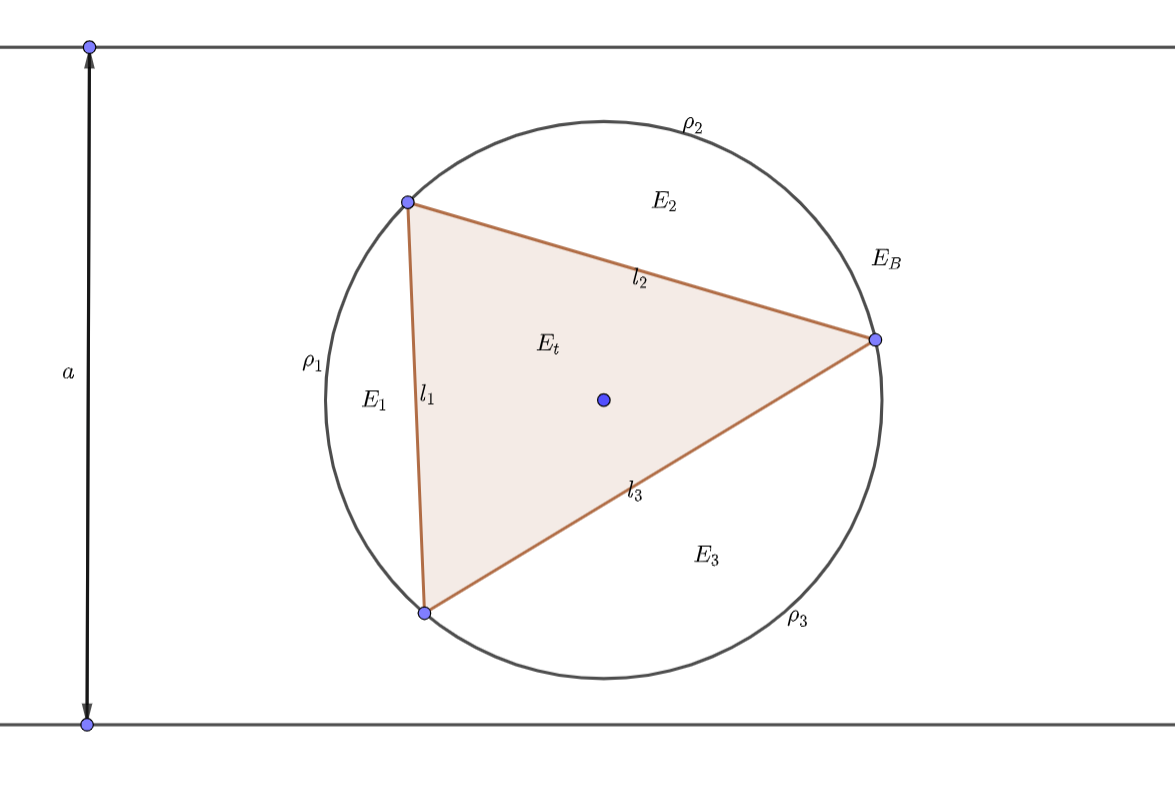
\includegraphics[width=0.8\textwidth]{figure.png}
}
% 表格模板
\renewcommand\arraystretch{0.8} % 设置表格高度为原来的0.8倍
\begin{table}[!htbp] % table标准
    \centering % 表格居中
    \begin{tabular}{p{1cm}<{\centering}p{1cm}<{\centering}p{3cm}<{\centering}p{5cm}<{\centering}} % 设置表格宽度
    %\begin{tabular}{cccc}
        \toprule
        $x_i$ & $f[x_1]$ & $f[x_i,x_{i+1}]$ & $f[x_i,x_{i+1},x_{i+2}]$ \\
        \midrule
        $x_0$ & $f(x_0)$ &                  &                          \\
        $x_0$ & $f(x_0)$ & $f'(x_0)$        &                          \\
        $x_0$ & $f(x_1)$ & $\frac{f(x_1)-f(x_0)}{x_1-x_0}$ & $\frac{f(x_1)-f(x_0)}{(x_1-x_0)^2}-\frac{f'(x_0)}{x_1-x_0}$\\
        \bottomrule
    \end{tabular}
\end{table}

\def\Log{\text{Log}} % 一个简单的宏定义
$\Log$ % 调用方法
\fi

\end{document}